\section*{Methods}

The focus of this study is regional accessibility for road vehicles. The metric developed reflects the time-cost for drivers in a region to access population centers within the region from one-another. It is important to consider total trip time. A sufficiently long trip will require at least one re-supply (refuel or recharge) event which adds to total trip time. In addition to the time required to re-supply the vehicle, there will be the time required to deviate from the shortest path to the supply station and  time spend waiting for an available port, time spent setting up the supply event. Before setting out for a trip, a driver will have limited and approximate information with which to plan a route. Drivers are faced with two related informational problems:

\begin{description}
	\item[Uncertainty] The driver may not know the instantaneous status of a given supply port.
	\item[Latency] The status of a supply port may change before the driver arrives.
\end{description}

Informational issues are particularly relevant for \gls{bev} drivers because of the relatively long duration of charging sessions compared to fueling sessions and the relative immaturity of the DC charging network as compared to the petroleum fueling network. For \gls{bev} drivers the variance in possible trip total time can be meaningful necessitating an earlier departure or other adjustment. As the journey progresses variance decreases. The routing methodology developed in this section reflects the informational difficulties facing \gls{bev} drivers. These are not helped by the fragmentary charging information space where network operators often guard status information and reservation capability within their proprietary apps if these are provided at all.

Regional characteristics determine how important the differences between vehicles and supply networks are. The land-use within a region has two principle effects. First, for a multi-city region, peripheral cities should experience worse regional access than central cities. Second, geographically large and/or sparse regions should experience worse overall accessibility than compact regions. Non-vehicular travel modes will vary by region and may take load away from the vehicular transportation system. Where only vehicular travel is concerned, mode choice is reduced to vehicle choice.

\subsection*{Metric Definition}

Regional travel is often modeled using gravity models. Gravity models theorize that the degree of connectivity between two entities is in proportion to the attractiveness of each and the difficulty-of-travel or impedance between them. Fitting such a model requires substantial and granular observed trip data not often available to the public. Impedance modeling (the denominator) is a key element of transportation demand modeling and is the focus of this study.

Being concerned with regional performance, this study proposes the regional impedance metric $Z_R$ which is a weighted mean of impedance. For region $R$ of $N$ nodes $O = \{O_1, O_2, \dots, O_N\}$ and a corresponding set of weights $W = \{W_0, W_1, \dots, W_N\}$, $G_R$ is computed as

\begin{equation}
	Z_{R} = \frac{1}{N^2}\sum_{i = 0}^{N} \sum_{j = 0 }^{N} Z_{ij} \label{eq:regional_impedance}
\end{equation}

for region $R$. Regional impedance as experienced at a specific origin $Z_{R,i}$ is defined as

\begin{equation}
	Z_{R,i} = \frac{1}{N}\sum_{j = 0 }^{N} Z_{ij} \label{eq:specific_regional_impedance}
\end{equation}

for origin $i$. $Z_R$ is a useful single-number metric for comparing the experience of travel in a region for different people living in different places and with different modes available to them. The variation within a region can be expressed using any metric of statistical dispersion such as standard deviation, Gini coefficient of inequality, etc.

\subsection*{Metric Computation}

In order to traverse an \gls{od} arc whose energy requirement is greater than a vehicle's \gls{ess} capacity, the vehicle must be re-supplied. Drivers will hold energy in reserve limiting a vehicles practical range in most cases. Because supply events add time to a trip, they will be minimized where possible \cite{Ge_2022}. For \glspl{icev}, supply events are brief and supply stations are ubiquitous in most areas. Routing services often neglect refueling events. For \glspl{bev}, supply events are lengthy and DC charging stations are not ubiquitous in most areas.  For this reason, dedicated \gls{bev} routing services such as A Better Route Planner and Tesla's UI compute routes which include supply events.

All drivers deal with uncertainty and latency issues when computing an optimal route. Rational drivers will plan a route based on some expectation of the many outcomes which contribute to travel cost. Traffic, availability of re-supply, and vehicle range are important factors as is the risk attitude of the driver. This mental process is modeled via stochastic optimization.

\subsubsection*{Stochastic Optimal Routing}

The purpose of stochastic optimal routing is to find lowest-expected-cost paths from origin $i \in V$ to a set of destinations $D \in V$ on graph $G = \{V, E\}$. The output is tree $P$ containing the optimal-feasible paths from the origin to the selected destinations. The objective of routing on arc $(i,j)\ i, j \in V$ is

\begin{equation}
	\min_{U \in \overline{U}_{i,j}}\ \mathbb{E}[J(S_0, U)]
\end{equation}

where

\begin{equation}
	J(U) = \sum_{k = 0}^M \Phi_k(S_0, U)
\end{equation}

s.t.

\begin{gather}	
	b^k_l \leq \mathbb{E}\left[\int_0^t \Phi_k(S_0, U)dt\right] \leq b^k_u\\
	\mathbb{E}\left[\int_0^T \Phi_k(S_0, U)dt\right] \geq b^k_f\\
	t \in [0, T]\quad k = 1, 2, \dots, M
\end{gather}

\noindent where $T$ is the final value of time for a route, $S$ is the state vector of $M$ states, $S_0$ is the initial values of the states, $U$ is a path between $i$ and $j$, $\overline{U}_{i,j}$ is the set of possible paths between $i$, and $j$, $\Phi$ is the set of cost functions, $b^k_l$ and $b^k_u$ are the upper and lower bounds for state $k$ respectively, and $b^k_f$ is the final state minimum value for state $k$. $\mathbb{E}$ denotes an expectation. State vector $S$ is initialized and stored as vectors containing $N$ discreet variables. A distribution $D$ for a the state vector at any node and time-step can be computed from a histogram of the values. Routes are considered feasible if state expectations remain within set bounds. Comparison between routes is performed using cost expectation. the goal of the optimization is to find the optimal path $U_{ij}^*$ such that $J(U_{ij}^*)$ is equal to the global minimum cost $J_{ij}^*$ for each arc $(i,j)\ i,j\in V$.

Th study assumes that drivers will attempt to minimize total trip time while maintaining a level of reserve energy determined by their risk tolerance. In theory, it is possible to traverse all \gls{od} arcs where both are connected to the road network. In practice certain arcs will be infeasible with this subset varying by driver. The structure of the optimization process is as follows. First, a graph is created to represent the supply network and its interactions among itself and with origins and destinations of interest. This graph is referred to as the \gls{sng} herein. All arcs which are feasible should be included as edges in the \gls{sng}, including those directly between origins and destinations. Second, edge costs in terms of total-time are assigned, using the driver, vehicle, and supply station models as described in the following subsections. Third, stochastic optimization is performed using an optimal routing algorithm based on the expectation of edge cost. Because this study concerns finding optimal paths for all pairs in a large set of locations, the Floyd-Warshall algorithm is used \cite{Floyd_1962, Warshall_1962}.

\subsubsection*{Driver Model}

Different drivers will have different perceptions of cost for the same information based on their priorities and risk attitudes. Drivers will prioritize factors such as time, money, distance, and complexity differently. In this study, drivers are assumed to only consider total trip time. Where any important factor is not known precisely drivers will consider a range of outcomes and decide based on an expectation. The result will be cost distribution $D$. Driver risk attitude concerns what range of outcomes will be used to compute expected cost. Risk attitude is modeled using a superquantile risk function defined as

\begin{equation}
	S(D, p_0, p_1) = \frac{1}{p_1 - p_0}\int_{p_0}^{p_1}Q(D, \alpha)\ d\alpha \label{eq:superquantile}
\end{equation}

\noindent where $p_0$ and $p_1$ are the boundaries of the range of probabilities considered in the expectation and $Q$ is the quantile function of $D$. The superquantile is the mean value of a distributed quantity within a range of probability. $S(D, 0, 1)$ reduces to the mean of $D$. Drivers with an aggressive risk attitude will consider the least costly outcomes. Drivers with a neutral attitude will consider central outcomes. Drivers with a cautious attitude will consider the most costly outcomes.

Drivers will desire to keep a minimum amount of range in reserve in any circumstance. This value is referred to as $SOC_{min}$. In practice, drivers may want to increase $SOC_{min}$ when operating in areas where supply infrastructure is sparsely distributed such that a backup station can be reached should the intended station not be usable. This behavior is modeled as the driver should arriving at a given station with enough remaining range to make it to at least three alternate stations. Thus, $SOC_{min}$ at each station is increased by the distance from the station to the third closest adjacent station. Driver parameters are listed in Table \ref{tab:param_driver}.

\begin{table}[H]
	\centering
	\caption{Driver Parameters for Routing}
	\label{tab:param_driver}
	\begin{tabular}{|C{\linewidth*3/8}|C{\linewidth*3/8}|C{\linewidth*2/8}|}
		\hline \rowcolor{lightgray} Parameter & Description & Unit \\
%		\hline Priorities $\Omega$ & Set of multipliers for route costs to be used in computation of composite cost & [-] \\
		\hline Risk Attitude $(p_0, p_1)$ & Range of probabilities for superquantile function & [-] \\
		\hline \gls{soc} Reserve $SOC_{min}$ & The lowest point of \gls{soc} that the driver will accept before re-supplying & [-] \\
		\hline
	\end{tabular}
\end{table}

\subsubsection*{Vehicle Model}

Vehicles effect routing due to their range limits and supply methods. The vehicle model used herein is highly simplified due to the inexact nature of the problem. Vehicles are modeled as storing energy and consuming energy at a constant rate per unit distance driven. More exact information on road conditions, traffic conditions, and atmospheric conditions among others can be used to compute edge-specific efficiencies. Vehicular parameters are listed in Table \ref{tab:param_veh}.

\begin{table}[H]
	\centering
	\caption{Vehicle Parameters for Routing}
	\label{tab:param_veh}
	\begin{tabular}{|C{\linewidth*3/8}|C{\linewidth*3/8}|C{\linewidth*2/8}|}
		\hline \rowcolor{lightgray} Parameter & Description & Unit \\
		\hline \gls{ess} Capacity & Accessible energy storage capacity & [kWh] \\
		\hline Energy Consumption & Energy required to move the vehicle & [kJ/km] \\
		\hline Maximum Supply Rate & \gls{ess} maximum energy addition rate & [kW] \\
		\hline Linear Charging Fraction & Percentage of the battery capacity which can be charged in the linear (constant current) range & [kW] \\
%		\hline \gls{soc} Bounds & Range in which \gls{soc} must be maintained & [-] \\
		\hline
	\end{tabular}
\end{table}

DC charging is modeled using a CC-CV relationship where the first part of charging is linear and the second part follows exponential decay \cite{Marra_2012}. The inflection point which separates the linear and exponential decay sections is the Linear Charging Fraction $\eta$. The time required for a given charge event is

\begin{gather}
	\Delta T = \Delta T_{l} + \Delta T_{e} \\
	\Delta T_{l} = \begin{cases}
		\frac{(SOC_f - SOC_i) C}{\nu} &  SOC_i \leq SOC_f \leq \eta \\
		\frac{(\eta - SOC_i) C}{\nu} &  SOC_i \leq \eta \leq SOC_f \\
		0 &  \eta \leq SOC_i \leq SOC_f
	\end{cases} \\
	\Delta T_{e} = \begin{cases}
		0 & SOC_i \leq SOC_f \leq \eta \\
		-\frac{1}{\alpha}\ln{\left(1-\frac{SOC_f - \eta}{1-\eta}\right)} &  SOC_i \leq \eta \leq SOC_f \\
		-\frac{1}{\alpha}\ln{\left(1-\frac{SOC_f - SOC_i}{1-\eta}\right)} &  \eta \leq SOC_i \leq SOC_f \\
	\end{cases} \\
	\alpha = \frac{\nu}{\eta C}
\end{gather}

Where $C$ is the vehicle \gls{ess} capacity, $\nu$ is the actual power of the charge event, $\Delta T_l$ and $\Delta T_e$ are the time spent in the linear and exponential decay portions of the charge event, and $SOC_i$ and $SOC_f$ are the initial and final values of \gls{soc} for the charge event. Charge events are modeled to occur at the minimum of the maximum powers for the vehicle and charger. A typical value for $\eta$ will be in the range of 0.7 to 0.8. DC charging for a given quantity of energy past $\eta$ will take substantially longer than the same quantity below $\eta$. The difference in effective charging rate may serve to favor more DC charge events each terminating at a lower \gls{soc}.

\subsubsection*{Supply Station Model}

Supply station parameters are number of ports, reliability of ports, and the maximum supply rate of ports. The probability of port availability at a station is determined by the rate at which vehicles arrive at the station and how long they spend at the station. In combination, these factors determine the likelihood of a port being usable and available as well as the likely duration of queue if no port is usable and available. Supply station parameters are listed in Table \ref{tab:param_supply}.

\begin{table}[H]
	\centering
	\caption{Supply Station Parameters}
	\label{tab:param_supply}
	\begin{tabular}{|C{\linewidth*2/8}|C{\linewidth*3/8}|C{\linewidth*3/8}|}
		\hline \rowcolor{lightgray} Parameter & Description & Unit \\
		\hline Supply Rate & Maximum rate of energy supply & [kW] \\
		\hline Ports & Number of chargers/pumps at a station which can be used simultaneously & [-] \\
		\hline Reliability & Percentage of the time that a given pump will be usable & [-] \\
		\hline Demand Level $\xi$ &  Non-dimensional parameter for station demand distribution. & [-] \\
		\hline
	\end{tabular}
\end{table}

Information on ports is taken from \gls{afdc} \cite{afdc_2023}, information on equipment reliability is taken from \cite{Rempel_2023}, and information on port supply rates is taken from Google Maps.

Queue waiting time is computed using the M/M/c queuing formula with parametric uncertainty. The expected waiting time in an M/M/c queue is computed as

\begin{gather}
	W_q = \pi_0\frac{\rho(c\rho)^c}{\lambda(1-\rho)^2c!}\\
	\pi_0=\left[\left(\sum_{k = 0}^{c - 1}\frac{(c\rho)^k}{k!}\right) + \frac{(c\rho)^c}{c!(1 - \rho)}\right]\\
	\rho = \frac{\lambda}{c\mu}
\end{gather}

where $\lambda$ is the arrival frequency, $\mu$ is the service completion frequency, $c$ is the number of homogeneous servers, $\rho$ is the ratio of arrival frequency to composite maximum service completion frequency, and $\pi_0$ is the probability of an empty system. One can think of $\rho$ as equivalent to "utilization". Where $\rho$ is low the station has excess capacity and where high the station is saturated. The expected waiting time in a M/M/c queue can be mapped for values of $\rho$ and $c$ as in Figure \ref{fig:reduncancy_rho_wq}.

\begin{figure}[H]
	\centering
	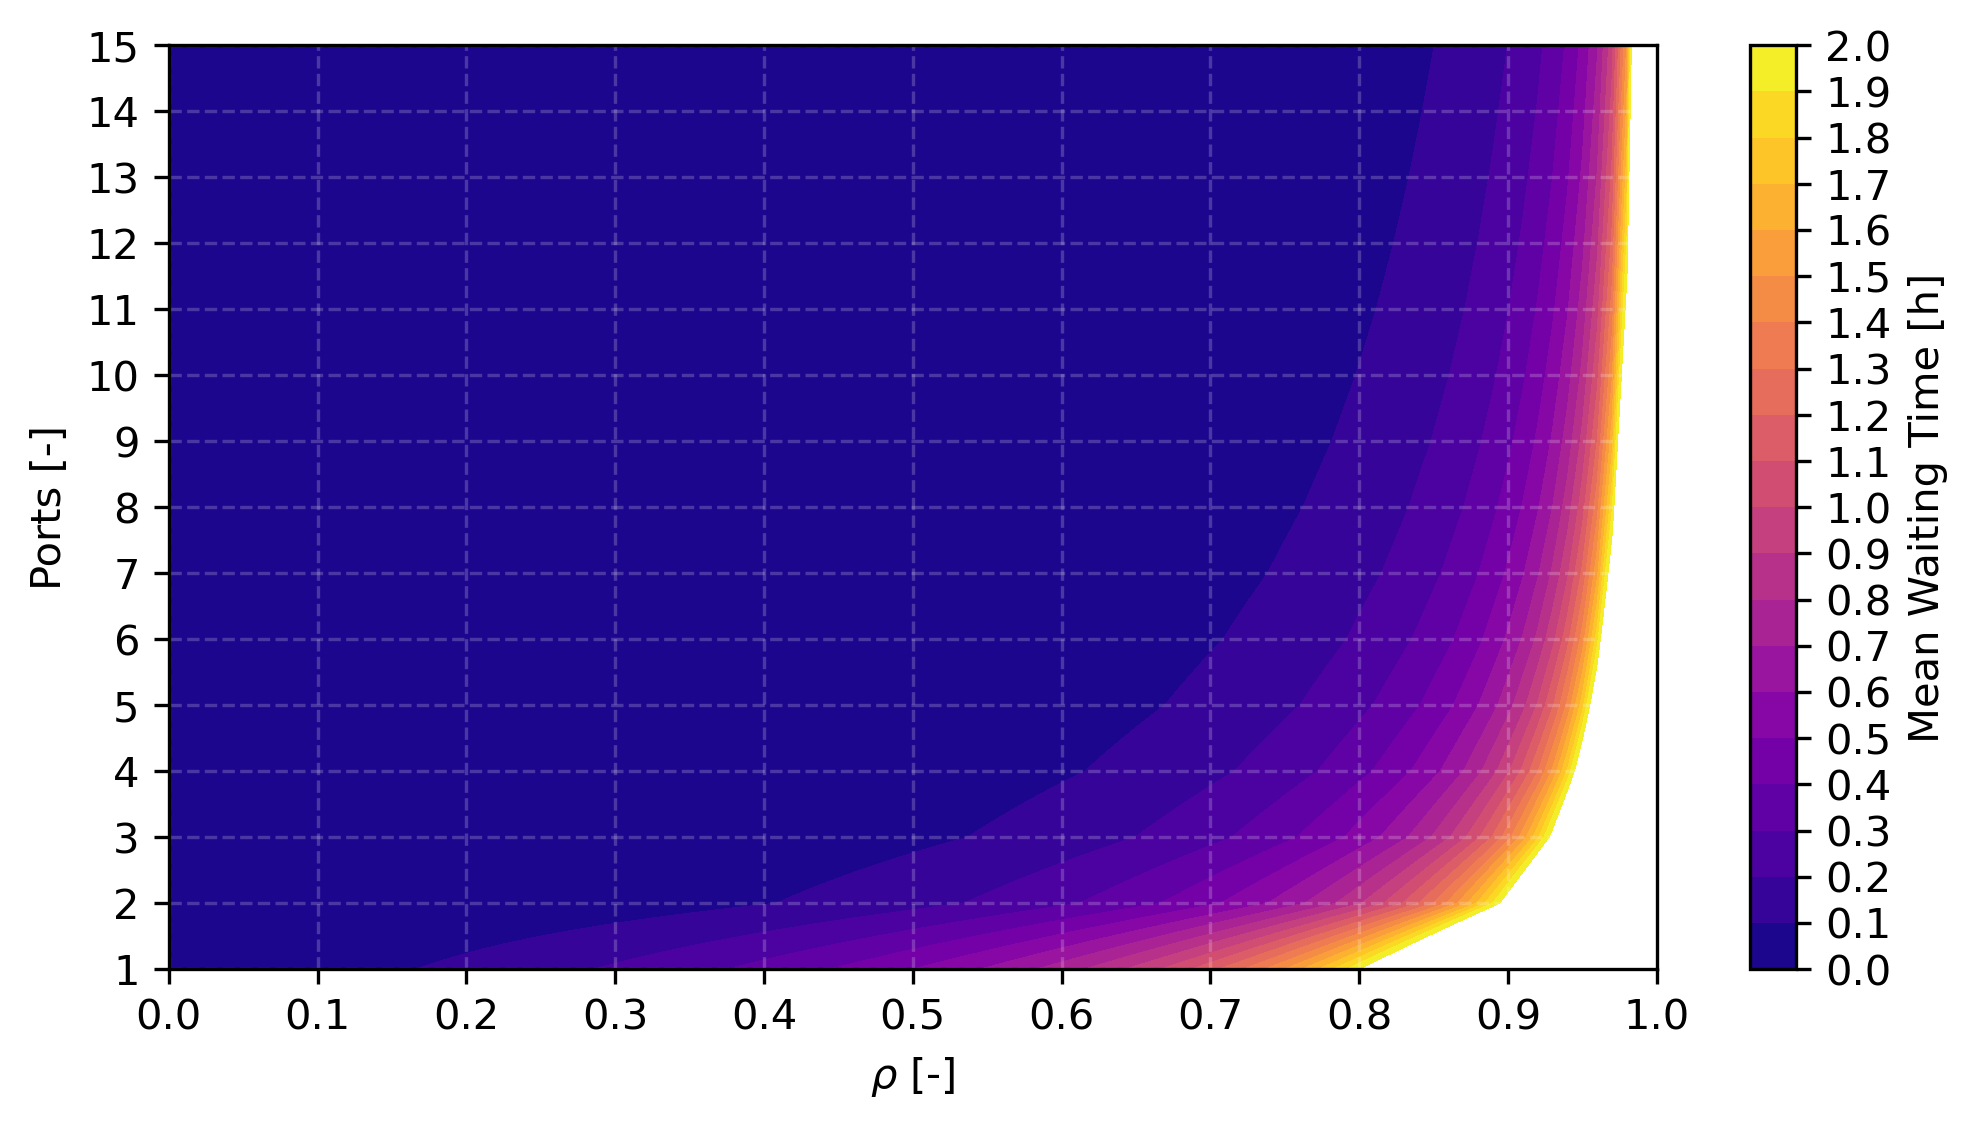
\includegraphics[width = \linewidth]{figs/waiting_time_rho_ports.png}
	\caption{Effects of in-station redundancy and $\rho$ on expected waiting time. Projected times of greater than 2 hours omitted in order to preserve scale.}
	\label{fig:reduncancy_rho_wq}
\end{figure}

The main implication of queue dynamics is that stations with more chargers will handle equivalent levels of utilization with shorted queues. The reason for this is that not all sessions will be of the same length and more chargers allows for further de-coordination of session start and end times.

Having a good idea of values for $\mu$ and $c$, the remaining parameter to estimate is the arrival rate $\lambda$. The driver will be aware that demand for transportation is likely to change with time-of-day, day-of-week, season, and on special occasions. An experienced driver should have some idea of how busy stations are likely to be based on experience and on road traffic volumes. In this study driver estimates of $\rho$ are sampled from Beta distribution where $2\leq \alpha \leq 4$ and $\alpha + \beta = 6$. PDFs for the distribution are shown in figure \ref{fig:rho_distributions}. The distirbution is parameterized by a singe variable $\xi\in [0, 1]$ where $\xi = .5 (\alpha - 2)$.

\begin{figure}[H]
	\centering
	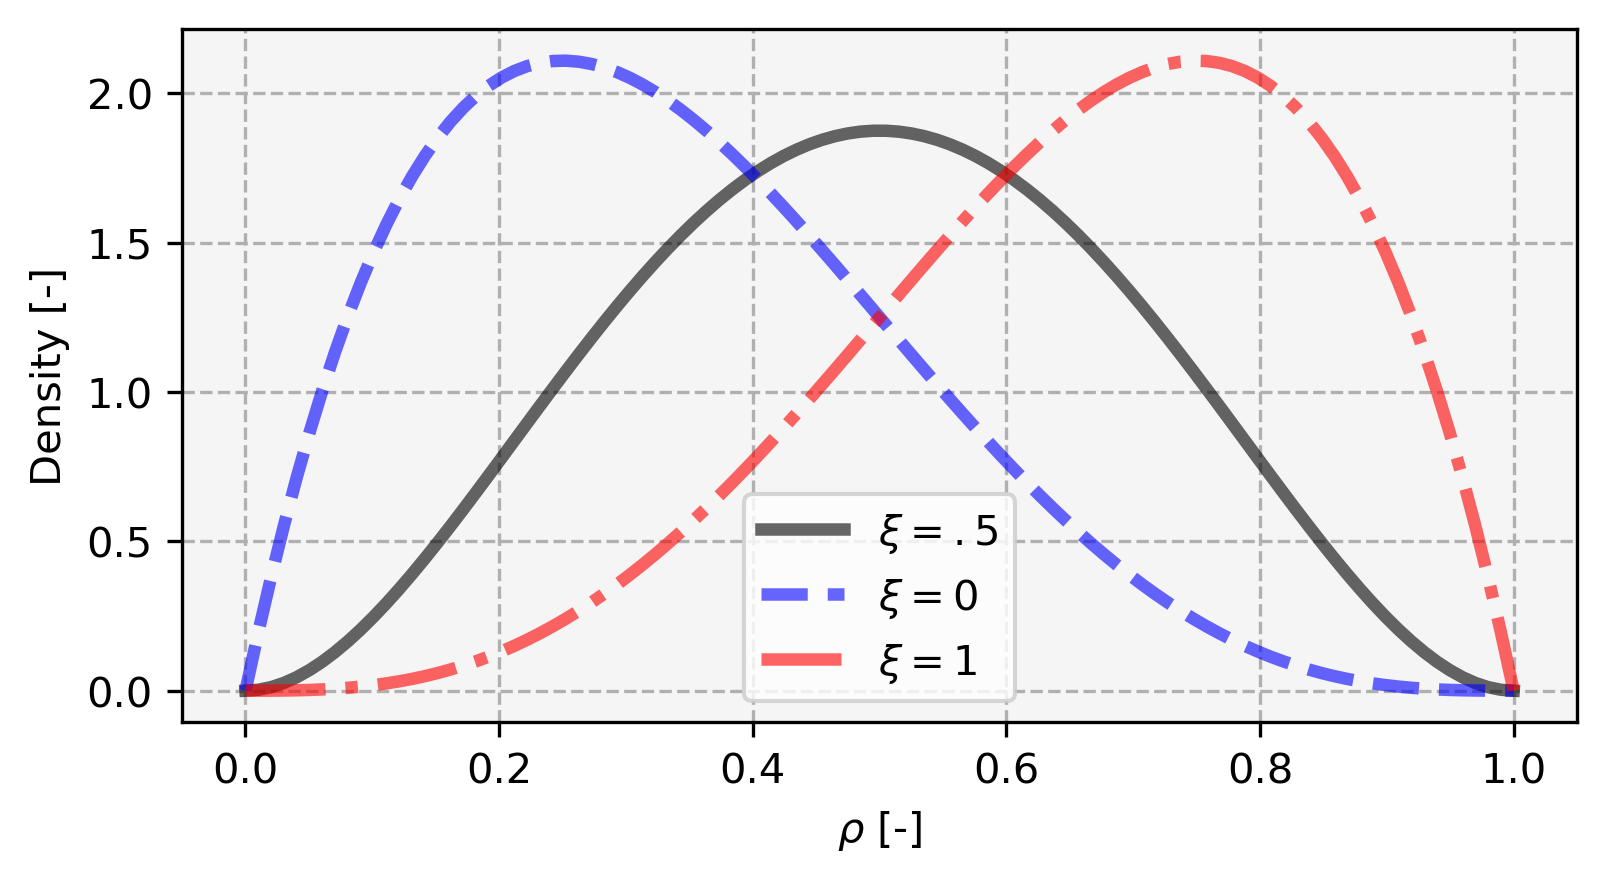
\includegraphics[width = \linewidth]{figs/rho_distributions.png}
	\caption{PDFs for $\rho$ Beta distributions reflecting low, medium, and high demand conditions.}
	\label{fig:rho_distributions}
\end{figure}

Thus, based on informed but imprecise knowledge, the driver can plan a time-minimal route accounting for likely queuing times.